%% ============================================================
%% Chapter 4 - Design and Implementation Elements
%% ============================================================

\chapter{Design and Implementation}\label{chapter:4_Design}

This chapter describes the implementation used for Mandarin tone classification
on Polish learner speech. The system receives one learner utterance and assigns
it to one of five expert categories,
\(\mathcal{T}=\{T_1,T_2,T_3,T_4,T_{\mathrm{NS}}\}\), where
\(T_1\)--\(T_4\) are the four full Mandarin lexical tones and
\(T_{\mathrm{NS}}\) denotes a non-standard learner production outside those four
tones. Expert tone annotation is used as the training and evaluation target, so
the reported scores measure agreement with perceived learner production rather
than with the intended prompt tone.

The experiments compare six complete setups. Setup~1 is a ToneNet-style CNN
baseline. Setups~2--4 are Wav2Vec~2.0 systems with different adaptation routes.
Setups~5--6 use Chinese HuBERT-Large with two prediction heads. All SSL systems
share the same learner manifest format and the same speaker-disjoint
train/development/test split. The CNN baseline follows a separate random image
split, matching the ToneNet-style image-classification protocol rather than the
SSL evaluation protocol.

\section{Model Architectures}
\label{sec:design:models}

\subsection{CNN baseline}
\label{sec:design:models:cnn}

The CNN baseline treats tone classification as image classification over
low-frequency mel-spectrograms, adapted from the ToneNet formulation
\cite{gao2019tonenet}. Each recording is loaded as mono 16\,kHz audio, trimmed
for leading and trailing silence, and converted into a log-mel spectrogram with
64 mel bands restricted to 50--350\,Hz. The spectrogram is rendered as a
225\(\times\)225 RGB image.

\begin{figure}[H]
\centering
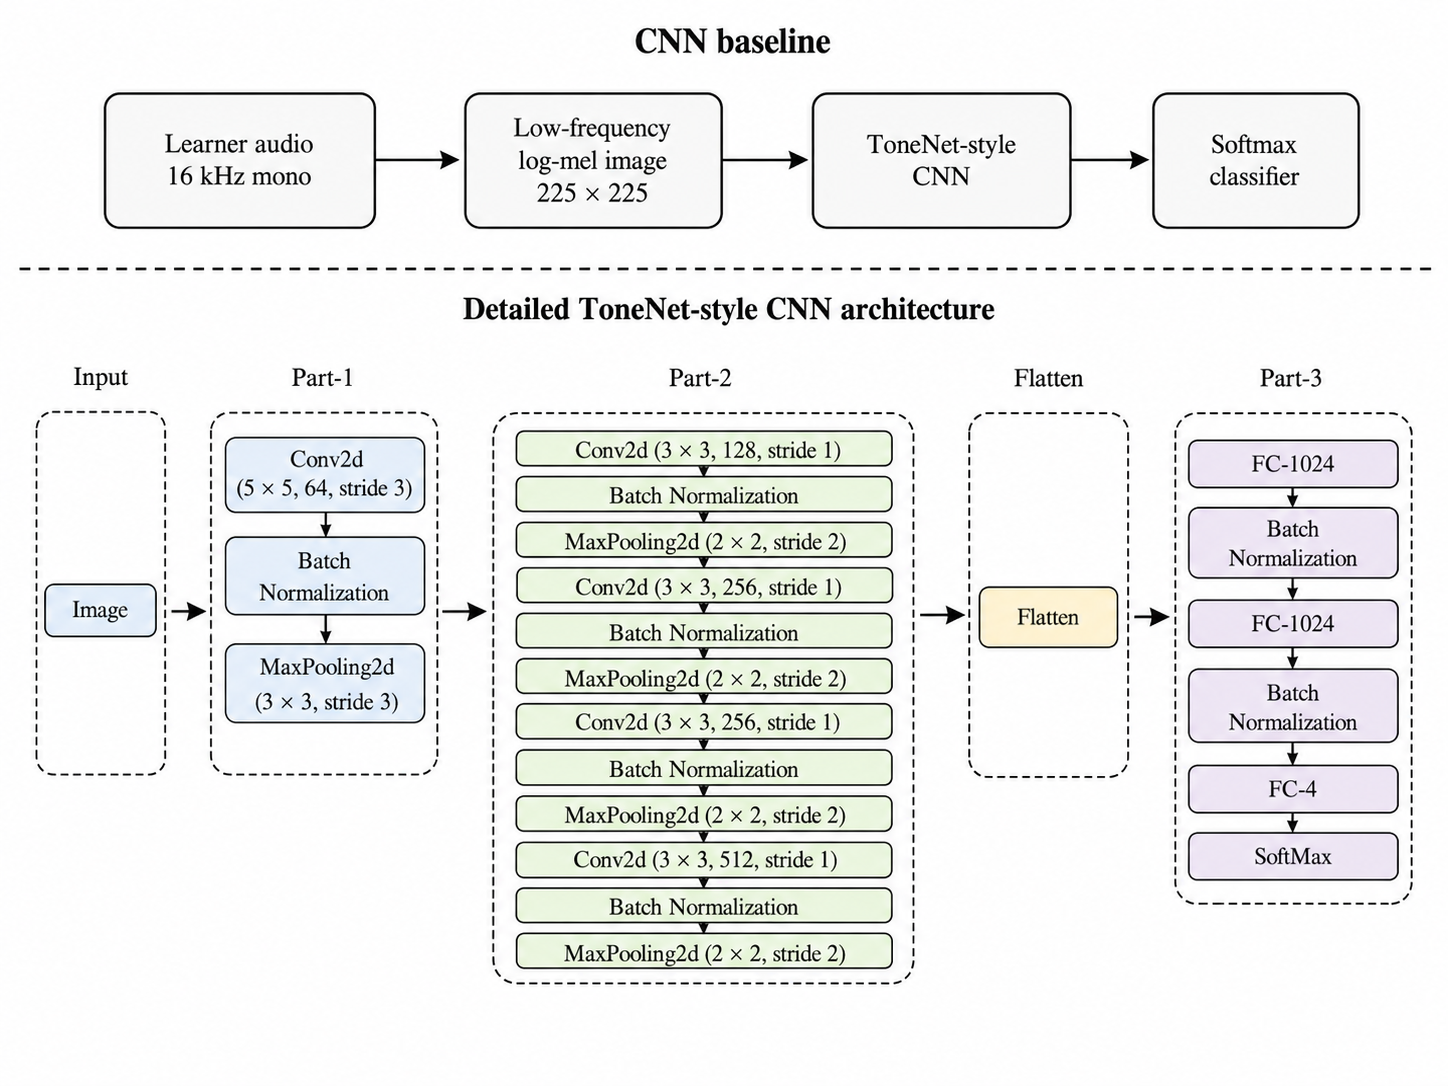
\includegraphics[width=\textwidth]{img/architecture/cnn_baseline.png}
\caption{CNN baseline architecture.}
\label{fig:design:cnn_arch}
\end{figure}

As shown in Figure~\ref{fig:design:cnn_arch}, the model first applies a
5 \(\times\) 5 convolution with 64 filters and stride 3, followed by batch
normalisation and max-pooling. Four VGG-style convolutional blocks then extract
higher-level image features. The final classifier contains two 1024-unit dense
layers and a five-class softmax output. The network is trained from scratch with
sparse categorical cross-entropy. Optimisation uses stochastic gradient descent
with learning rate 0.001, momentum~0.9, and Nesterov acceleration.

\subsection{Wav2Vec~2.0 fine-tuning}
\label{sec:design:models:wav2vec}

The Wav2Vec~2.0 experiments use three fine-tuning routes, shown in
Figure~\ref{fig:design:wav2vec_routes}. Setup~2 starts from the English
\mbox{wav2vec2-large-960h} checkpoint and fine-tunes directly on the
learner corpus \cite{baevski2020}. Setup~3 first trains the same checkpoint on
AISHELL-1 frame-level Mandarin tone labels for \(T_1\)--\(T_4\), excluding
neutral-tone and silence frames from the loss, and then fine-tunes the resulting
checkpoints on learner speech \cite{bu2017aishell}. Setup~4 starts from
\mbox{chinese-wav2vec2-large}, a Mandarin-specific checkpoint
pre-trained on WenetSpeech, and fine-tunes directly on learner speech
\cite{zhang2022wenetspeech,tencentgamemate2022}.

\begin{figure}[H]
\centering
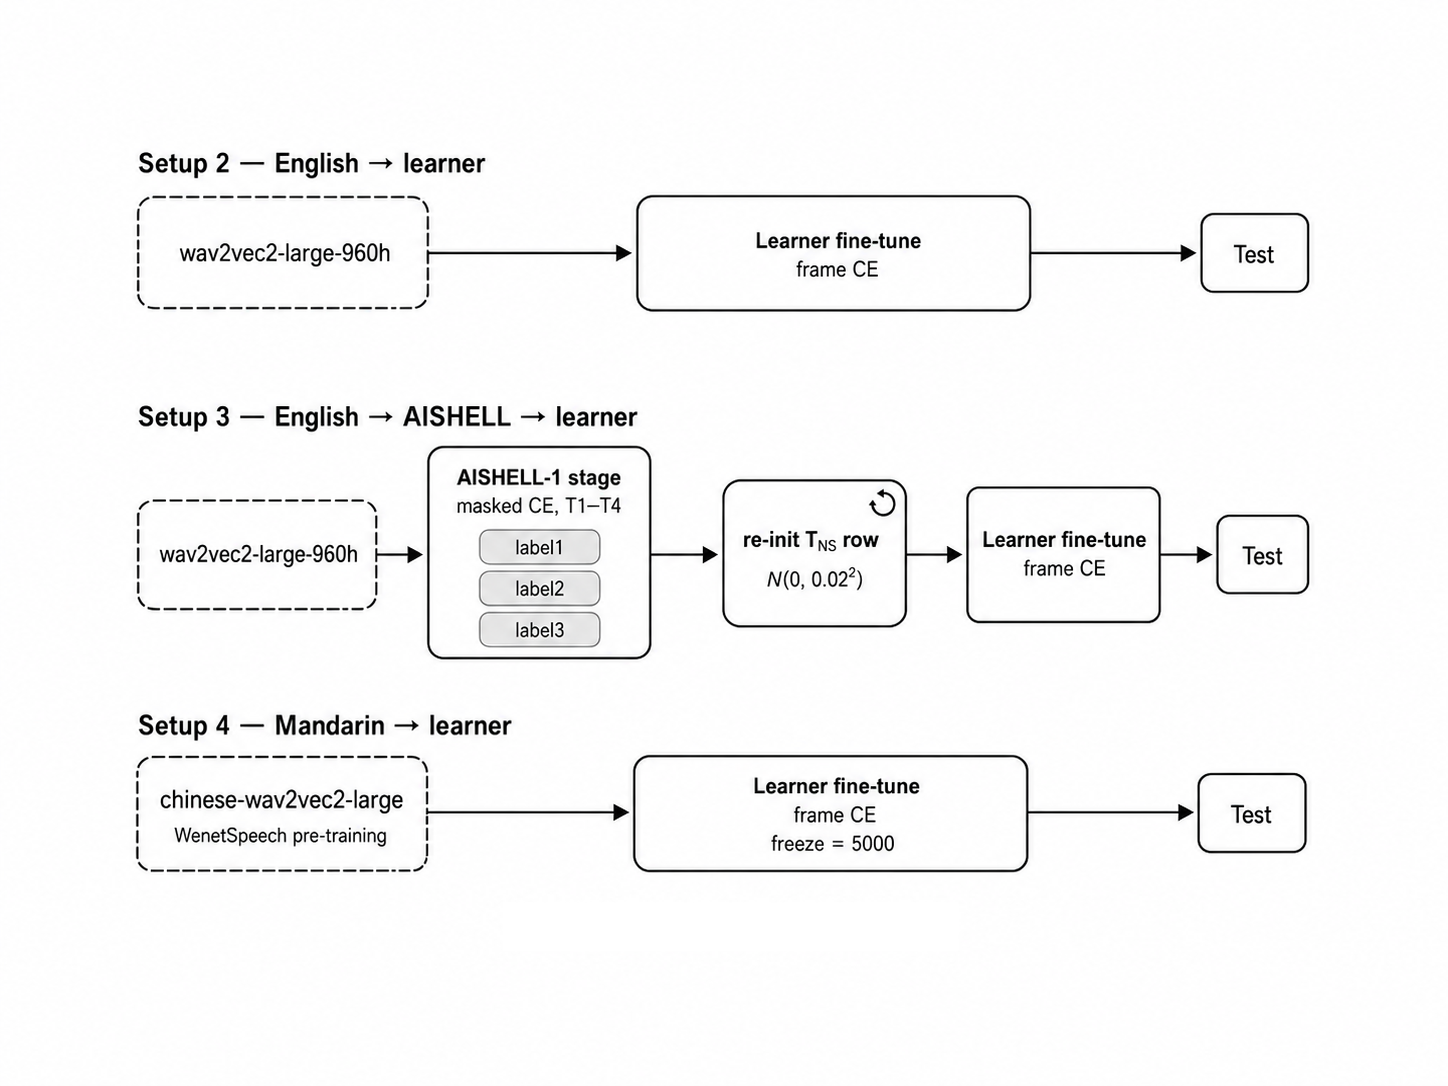
\includegraphics[width=\textwidth]{img/architecture/fig4_2.png}
\caption{Wav2Vec~2.0 fine-tuning routes.}
\label{fig:design:wav2vec_routes}
\end{figure}

All three routes use the common architecture in
Figure~\ref{fig:design:wav2vec_common}. The input is a 16\,kHz waveform. The
convolutional feature extractor remains frozen, while the Transformer encoder
provides hidden states \(h_{l,t}\) for layer \(l\) and frame \(t\). A trainable
layer-weight vector is normalised by softmax:
\begin{equation}
  \alpha_l = \frac{\exp(w_l)}{\sum_{j} \exp(w_j)}, \qquad
  h_t = \sum_l \alpha_l h_{l,t}.
  \label{eq:design:weighted_layer_sum}
\end{equation}
The weighted frame representation \(h_t\) is passed to a linear classifier.

\begin{figure}[H]
\centering
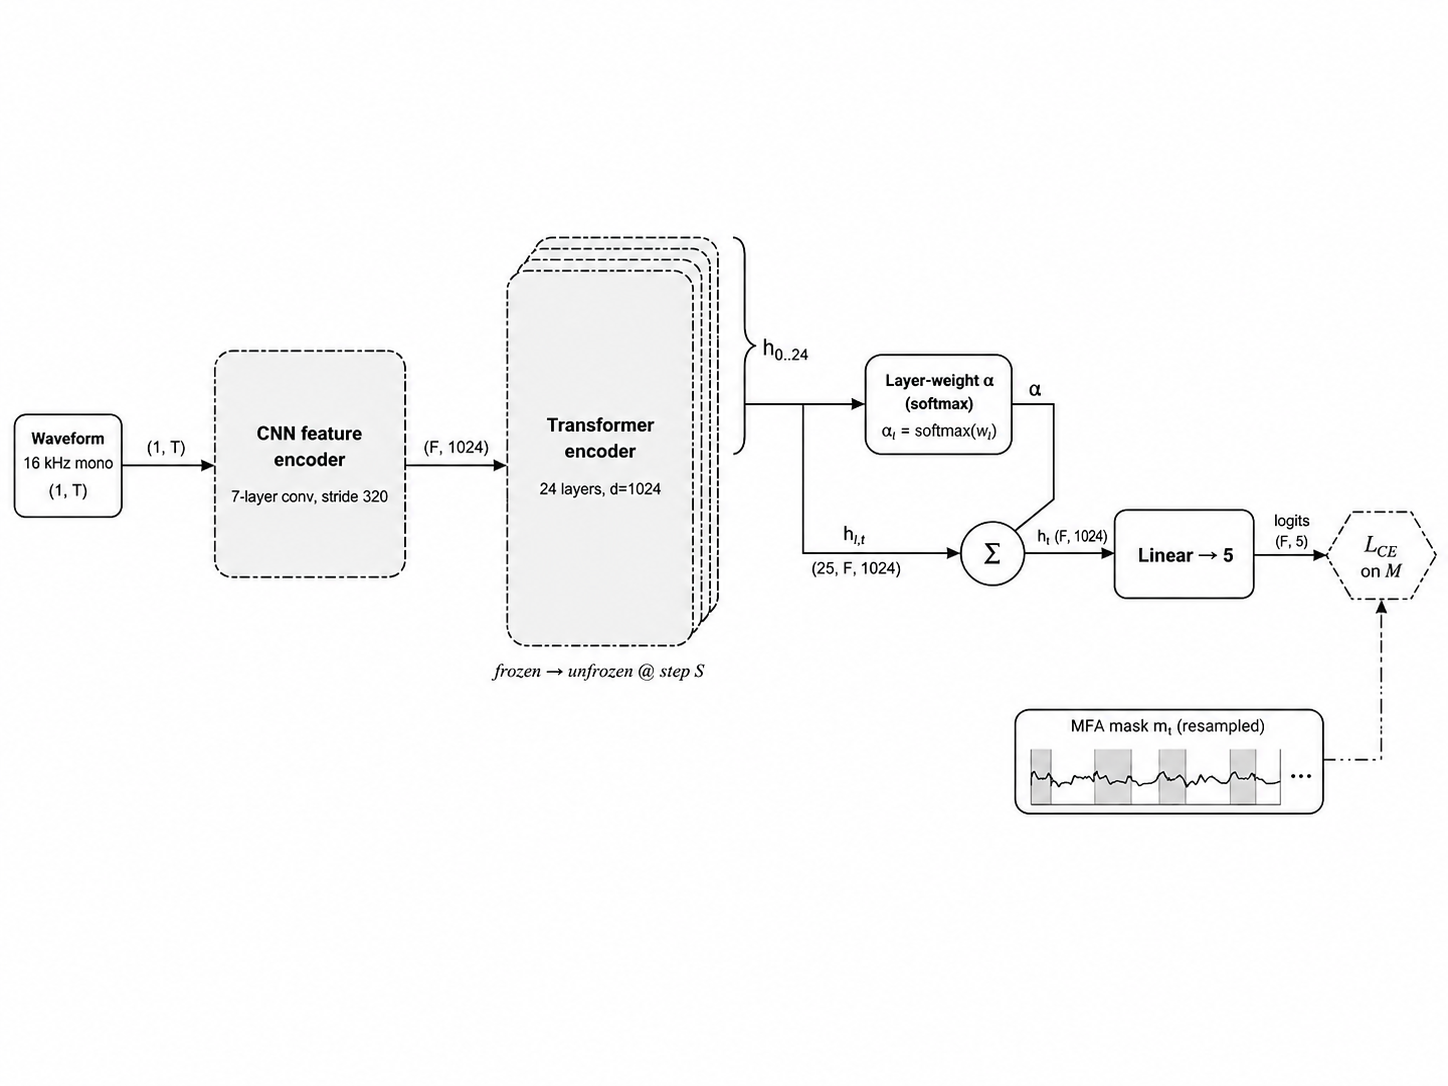
\includegraphics[width=\textwidth]{img/architecture/fig4_3.png}
\caption{Common SSL frame-level backbone.}
\label{fig:design:wav2vec_common}
\end{figure}

For learner fine-tuning, the utterance-level expert label is copied to the
speech frames selected by the MFA mask. Cross-entropy is computed only on these
frames:
\begin{equation}
  \mathcal{L}_{\text{CE}}
  =
  -\frac{1}{|M|}
  \sum_{t \in M}
  \log p(y \mid h_t),
  \label{eq:design:frame_ce}
\end{equation}
where \(M\) is the set of selected speech frames. During inference, each masked
frame votes for a tone category:
\begin{equation}
  \hat{y}
  =
  \argmax_{c \in \mathcal{T}}
  \sum_{t \in M} \mathbf{1}\!\left[\argmax_{k} p(k \mid h_t) = c\right].
  \label{eq:design:majority_vote}
\end{equation}
For both training and inference, if the resampled mask contains fewer than five
speech frames, all encoder frames are used.

For Setup~3, AISHELL-1 intermediate training uses MFA-derived frame-label
streams rather than copied learner labels. The best checkpoint for each stream
is selected by AISHELL-1 development frame accuracy computed over \(T_1\)--\(T_4\)
frames and then used to initialise learner fine-tuning.

\subsection{HuBERT fine-tuning}
\label{sec:design:models:hubert}

The HuBERT experiments use Chinese HuBERT-Large, another Mandarin-specific
checkpoint released from WenetSpeech pre-training
\cite{hsu2021,zhang2022wenetspeech,tencentgamemate2022}. Setup~5 uses the same
frame-level cross-entropy and majority-vote strategy as the Wav2Vec~2.0
systems. Setup~6 replaces frame voting with an utterance-level attention head.

In the attention variant, each speech frame receives a scalar attention score:
\begin{equation}
  e_t = v^\top \tanh(W h_t), \qquad
  a_t = \frac{\exp(e_t)m_t}{\sum_{\tau} \exp(e_\tau)m_\tau},
  \label{eq:design:attention_pool}
\end{equation}
where \(m_t\in\{0,1\}\) is the resampled speech mask. The utterance vector is
\begin{equation}
  z = \sum_t a_t h_t,
  \label{eq:design:utt_repr}
\end{equation}
and a linear classifier maps \(z\) to the five expert categories. The attention
variant uses focal loss with \(\gamma=2\)~\cite{lin2017focal}:
\begin{equation}
  \mathrm{FL}(p_y) = -\,{(1-p_y)}^{\gamma}\log p_y.
  \label{eq:design:focal}
\end{equation}

Both HuBERT variants keep the convolutional feature extractor frozen. Training
starts with the Transformer blocks frozen; only the layer weights and the tone
head are updated with learning rate \(1\times10^{-4}\). After 2{,}000
optimisation steps, the Transformer blocks are unfrozen and fine-tuned with
learning rate \(1\times10^{-5}\), while the convolutional feature extractor
remains frozen.

\begin{figure}[H]
\centering
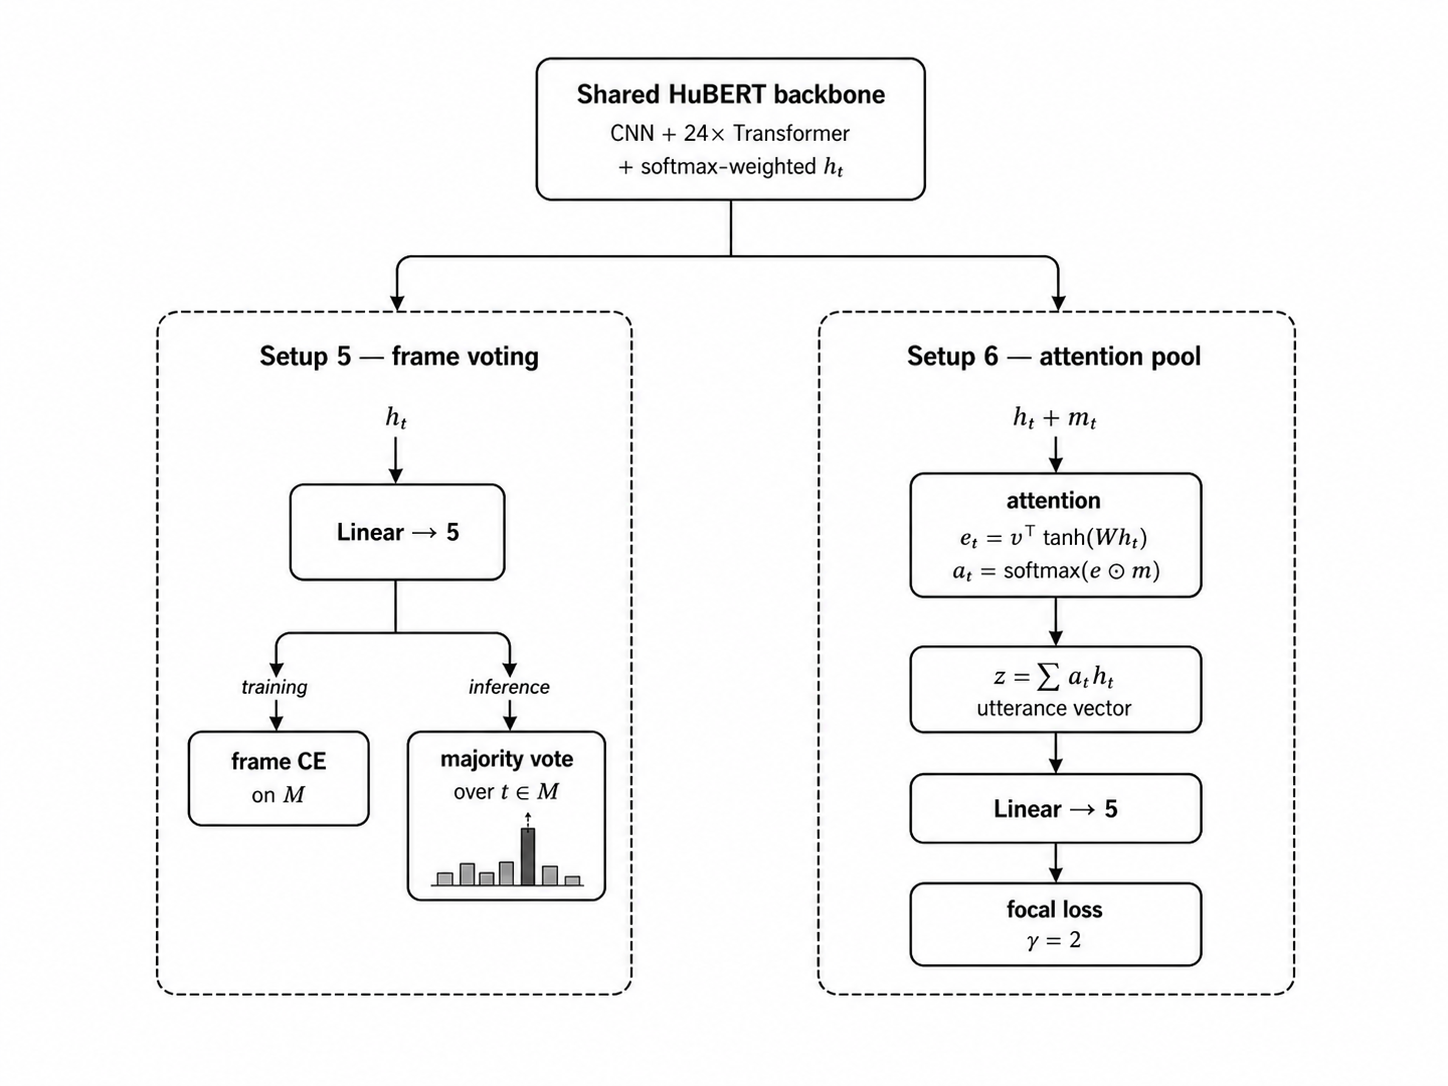
\includegraphics[width=\textwidth]{img/architecture/fig4_4.png}
\caption{HuBERT prediction heads.}
\label{fig:design:hubert_heads}
\end{figure}

\section{Data Preparation}
\label{sec:design:pipeline}

\subsection{Learner corpus}
\label{sec:design:pipeline:learner_database}

To make the evaluation reflect generalisation to unseen Polish learners, the
learner corpus was prepared with speaker separation as the main constraint. The
original assessment file contains 679 learner profiles collected in two recording
stages. Stage~I consists of isolated number-word productions, while Stage~II
contains everyday vocabulary and short phrase recordings. The expert annotation
uses tone value~0 when the learner production does not realise any well-formed
Mandarin tone and values~1--4 for perceived productions of the four full tones.
These labels are mapped to \(T_{\mathrm{NS}}\) and \(T_1\)--\(T_4\),
respectively. The value~0 is therefore a dataset-specific expert flag for a
non-standard production, not the linguistic neutral tone.

For the SSL experiments, each recording had to satisfy two requirements: an
expert tone rating had to be available in the assessment spreadsheet, and the
audio had to be successfully aligned by Montreal Forced Aligner~(MFA)
\cite{mcauliffe2017mfa}. Applying
these criteria produced the working learner corpus used by the frame-level
systems: 6\,623 Stage~I utterances and 4\,700 Stage~II utterances, giving
11\,323 utterances from 678 speakers. Each utterance is stored as a JSONL record
that links the utterance identifier with the waveform path, the binary speech
mask, and the expert tone label. The identifiers preserve both speaker identity
and prompt index, which makes it possible to combine the two stages while still
tracking the source of every item.

The corpus was then divided into training, development, and test partitions at
the speaker level. No speaker appears in more than one partition. This protocol
prevents the model from being evaluated on voices already seen during training
and makes the test scores a closer estimate of performance on new learners. The
final split contains 8\,577 training utterances, 464 development utterances, and
2\,282 test utterances. The development set is used for checkpoint selection,
whereas the test set is held out until the final evaluation reported in
Chapter~\ref{chapter:5_Experiments}.

MFA alignments are also used to define the speech regions for frame-level
training. Phone intervals from TextGrid files are projected onto a fixed 25\,ms
grid. A frame is marked as speech when it overlaps a non-silence phone interval;
otherwise it is excluded from the loss and from the majority-vote aggregation
used at inference time. This masking procedure also removes padding frames
introduced when short waveforms are batched.

\subsection{AISHELL-1 label streams}
\label{sec:design:pipeline:aishell}

Setup~3 adds an intermediate stage on native Mandarin read speech from
AISHELL-1. After MFA alignment, frames are labelled from the corpus phone
notation, but only frames corresponding to the four full tones
\(T_1\)--\(T_4\) are used as AISHELL supervision. Frames annotated as the
linguistic neutral tone, silence, consonant-only regions, or any other non-tone
class are mapped to the ignore index and excluded from the AISHELL loss. This
prevents the fifth learner output category from being trained to mean neutral
tone during native-speech adaptation. The three parallel label streams are
adapted from the design proposed by Yuan et~al.~\cite{yuan2023}: they reuse
the same waveforms and training hyperparameters but change where
\(T_1\)--\(T_4\) supervision is placed in time
(Table~\ref{tab:design:aishell_label_streams}).

\begin{table}[H]
\centering
\caption{AISHELL-1 frame-label streams.}
\label{tab:design:aishell_label_streams}
\small
\begin{tabular}{>{\raggedright\arraybackslash}p{0.18\textwidth} >{\raggedright\arraybackslash}p{0.72\textwidth}}
\toprule
\textbf{Stream} & \textbf{Rule} \\
\midrule
label1 & The tone label spans the toned rhyme and the preceding onset, so the whole syllable carries one tone class. \\
\addlinespace
label2 & Only the toned rhyme receives the tone label; the onset is assigned a non-tone label and excluded from the tone loss. \\
\addlinespace
label3 & Tone labels are attached only at the temporal midpoint of tone-bearing phones; consonants and other regions stay outside the tone objective. \\
\bottomrule
\end{tabular}
\end{table}

\begin{figure}[H]
\centering
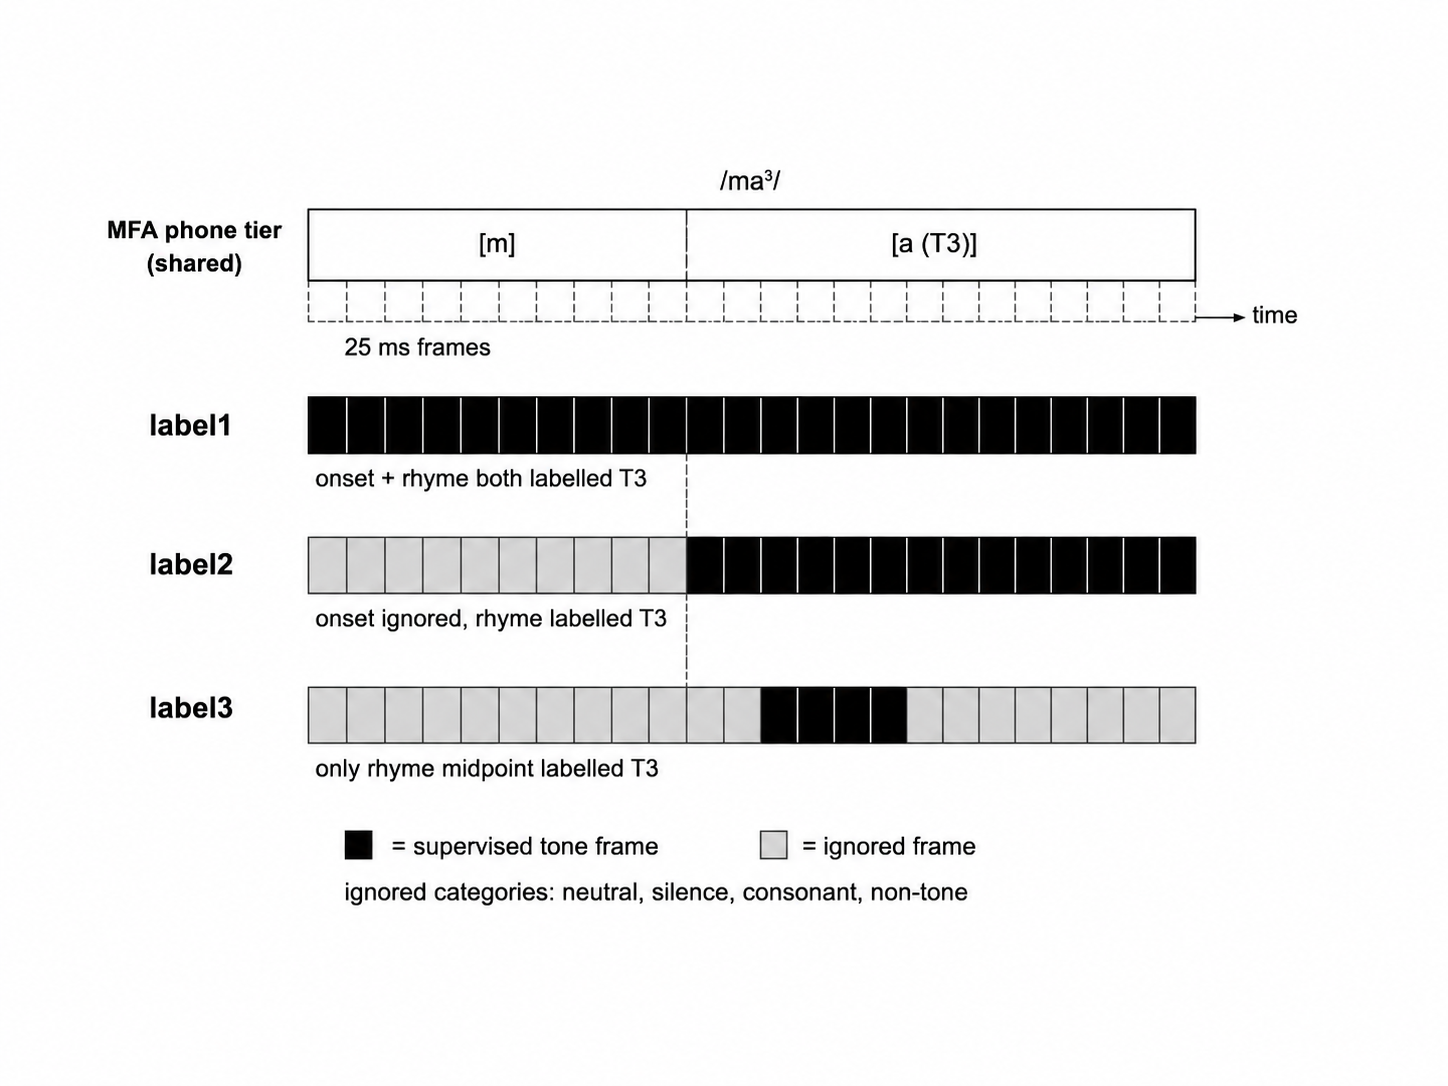
\includegraphics[width=\textwidth]{img/architecture/fig4_5.png}
\caption{AISHELL-1 frame-label streams.}
\label{fig:design:aishell_streams}
\end{figure}

After filtering and the train/dev partition used in the notebooks, the
intermediate AISHELL-1 stage trains on 33\,986 utterances and monitors a held-out
development set of 693 utterances. The AISHELL objective uses a masked
cross-entropy over only the first four logits:
\begin{equation}
  \mathcal{L}_{\text{AISHELL}}
  =
  -\frac{1}{|M_A|}
  \sum_{t \in M_A}
  \log
  \frac{\exp z_{t,y_t}}{\sum_{k=1}^{4}\exp z_{t,k}},
  \qquad y_t \in \{T_1,T_2,T_3,T_4\},
  \label{eq:design:aishell_masked_ce}
\end{equation}
where \(M_A\) excludes neutral-tone, silence, and non-tone frames. Because the
fifth learner category \(T_{\mathrm{NS}}\) is not part of the AISHELL softmax, it
receives no native-speech training signal. Before learner fine-tuning, the first
four classifier rows are copied from the AISHELL checkpoint, while the fifth row
for \(T_{\mathrm{NS}}\) is re-initialised from a Gaussian distribution with
mean~0 and standard deviation~0.02.

\subsection{CNN image features}
\label{sec:design:pipeline:cnn_features}

The CNN baseline bypasses raw waveforms and instead reads fixed-size images.
Because this branch does not require MFA alignment, its eligible set is larger
than the SSL working corpus. Every labelled learner recording is rasterised to
the same low-frequency
mel-spectrogram layout as in Section~\ref{sec:design:models:cnn}, exported as a
PNG, and stacked into a cache of 11\,934 tensors with spatial size 225 by 225
and three colour channels.
Figure~\ref{fig:design:cnn_mel_examples} shows five illustrative crops after this
rendering pipeline (Tone~0 denotes the non-standard \(T_{\mathrm{NS}}\) category;
Tone~1--Tone~4 correspond to \(T_1\)--\(T_4\)); subtitles record learner utterance
identifiers from the corpus.

\begin{figure}[H]
\centering
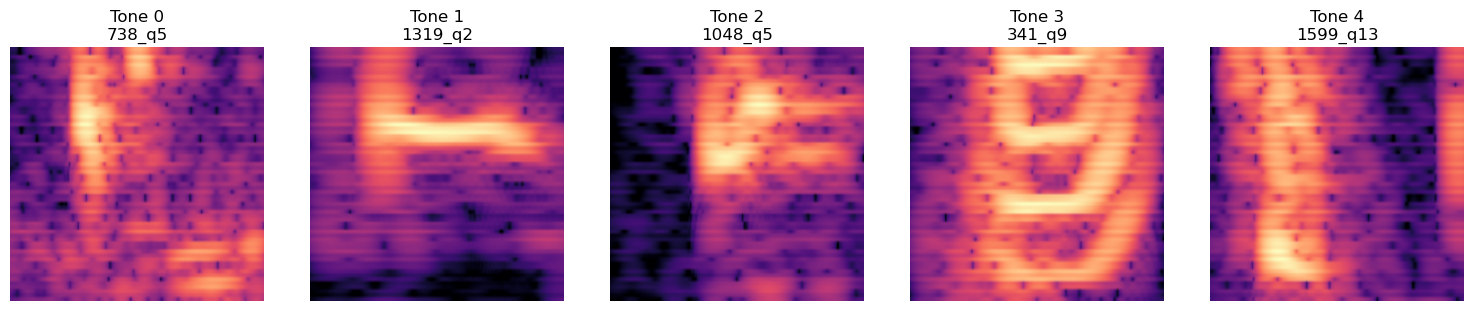
\includegraphics[width=\textwidth]{img/experiments/mel_example.png}
\caption{Low-frequency mel-spectrogram images used as CNN inputs.}
\label{fig:design:cnn_mel_examples}
\end{figure}

Images are split at random in the ToneNet style:
9\,546 training images, 1\,194 validation images, and 1\,194 test images.

\section{Training and Evaluation}
\label{sec:design:implementation}

The experimental code was organised as Jupyter notebooks. Each run saved the
checkpoints and learning curves needed to inspect the training process. MFA
supplies the phone alignments, while Librosa and Matplotlib are used for
exploratory audio and feature plots. The CNN baseline is implemented with
TensorFlow/Keras, and the SSL models are implemented with PyTorch and Hugging
Face Transformers.

For SSL training, each input is a mono 16\,kHz utterance and the batch size is
one utterance. Optimisation uses AdamW, gradient clipping at maximum norm~1.0,
and 1{,}000 warm-up updates. During the frozen phase, only the learned layer
weights and the tone-classification head are updated, using a learning rate of
\(1\times10^{-4}\). For Setups~3, 5, and~6, the Transformer layers are
unfrozen after 2{,}000 updates and training continues to 40{,}000 updates;
for Setups~2 and~4 the corresponding values are 5{,}000 and 30{,}000. The
schedule choice for each setup is justified in
Appendix~\ref{sec:app:sensitivity}. After unfreezing, the Transformer is
fine-tuned with learning rate \(1\times10^{-5}\), while the convolutional
feature encoder remains frozen.
Development evaluation is performed every 1{,}000 updates. Checkpoint selection
uses learner development accuracy for the frame-voting systems, learner
development macro-F1 for the HuBERT attention model, and native-speech
frame-level development accuracy for the AISHELL-1 intermediate stage.

MFA masks and AISHELL frame labels are stored on a 25\,ms grid, whereas
Wav2Vec~2.0 and HuBERT produce hidden states on the encoder time axis. The masks
and labels are therefore mapped to the encoder sequence length using
nearest-neighbour resampling. For a source sequence of length \(L\) and an
encoder sequence of length \(F\), encoder frame \(j\) receives source index
\begin{equation}
  i_j = \mathrm{round}\!\left(\frac{j(L-1)}{F-1}\right),
  \qquad j \in \{0,\dots,F-1\}.
  \label{eq:design:resample}
\end{equation}

The time- and feature-masking augmentations provided by the Hugging Face
implementations are disabled by setting the masking probabilities to zero. This
avoids removing a large proportion of the signal in short learner utterances.

The CNN hyperparameters follow the ToneNet-style image-classification recipe of
Gao et~al.~\cite{gao2019tonenet} where applicable. The SSL configuration uses
Wav2Vec~2.0 and HuBERT backbones~\cite{baevski2020,hsu2021}, AdamW
optimisation~\cite{loshchilov2019decoupled}, and the frame-level tone objective,
full fine-tuning learning rate, and AISHELL-1 label streams from Yuan
et~al.~\cite{yuan2023}. Values not fixed by those sources are listed in
Appendix~\ref{page:B_appendix}; the schedule-sensitive values are further
checked in the Optuna study in Appendix~\ref{sec:app:sensitivity}.

At the end of each experiment, the corresponding notebook saves a JSON summary
containing the split sizes, the best development score, test-set aggregate
metrics, per-category metrics, and the confusion matrix.
Chapter~\ref{chapter:5_Experiments} uses these summaries to construct the result
tables.



\section{Chapter Summary}
\label{sec:design:summary}

This chapter presented the model and data design used in the experiments. The
CNN baseline uses low-frequency mel-spectrogram images. The Wav2Vec~2.0 systems
share a frame-level task head but differ in their adaptation route. The HuBERT
systems compare frame-level voting with utterance-level attention pooling. All
SSL systems rely on MFA-derived masks, speaker-disjoint learner splits, and
saved JSON summaries for reproducible evaluation.
